\documentclass[a4paper]{article}
\usepackage[utf8]{inputenc}
\usepackage{amssymb}
\usepackage[ngerman]{babel}
\usepackage{hyperref}
\usepackage{enumitem}
\usepackage{listings}
\usepackage{amsmath}
\usepackage{esvect}
\usepackage{float}
\usepackage{graphicx}
\usepackage[table]{xcolor}% http://ctan.org/pkg/xcolor
\usepackage{todonotes}
\usepackage{pgfplots}
\usepackage{verbatim}
\usepackage{multirow}
\usepackage{booktabs}
\pgfplotsset{compat=1.10}
\usepgfplotslibrary{fillbetween}
\usetikzlibrary{patterns}
\usepackage{mathtools}
\usepackage{centernot}
\usepackage{mathabx}

\newcommand{\uproman}[1]{\uppercase\expandafter{\romannumeral#1}}
\newcommand\mathbfont{\usefont{U}{mathb}{m}{n}}

\hypersetup{
     colorlinks   = true,
     citecolor    = gray
}


\title{Grundlagen der Rechnerarchitektur Blatt 5}
\author{Marco Deuscher \and Carolin Schindler}
\date{27. November 2019}

\begin{document}

\maketitle
\section{Aufgabe: Was war nochmal der Unterschied..?}
Eine bool'sche Algebra ist ein komplementärer distributiver Verband $(B,+,\cdot,0,1)$ mit den Eigenschaften Assoziativität, Kommutativität, Idempotenz, Absorption und Distributivität.\\
Die Schaltalgebra ist eine bool'sche Algebra mit $B=\{0,1\}$.
\section{Aufgabe 2: Minimierung macht alles einfacher}
\paragraph{(a)}
\begin{align*}
	g(x_1,x_2)&= \overline{\overline{x_1x_2}x_1} \stackrel{\text{P8}}{=} \overline{(\overline{x_1}+\overline{x_2})\cdot x_1}  \stackrel{\text{P8}}{=}\overline{(\overline{x_1}+\overline{x_2})}+\overline{x_1}\\
			  &\stackrel{\text{P8'}}{=} (\overline{\overline{x_1}}\cdot \overline{\overline{x_2}}) + \overline{x_1} \stackrel{\text{P7}}{=} (x_1x_2)+\overline{x_1} \stackrel{\text{P4'}}{=} (x_1+\overline{x_1})\cdot(x_2+\overline{x_1}) \stackrel{\text{P9'}}{=} 1\cdot (x_2+\overline{x_1})\\
			  &\stackrel{\text{P5}}{=} x_2 + \overline{x_1}
\end{align*}
\paragraph{(b)}
\begin{align*}
	h(x_1,x_2,x_3,x_4) &= (x_1\cdot x_2)+(x_1\cdot x_3)+x_1(x_2+x_3\cdot x_4) + x_1 \\
					   &\stackrel{\text{P5}}{=} (x_1x_2)+(x_1x_3)+x_1(x_2+x_3x_4)+x_1\cdot 1\\
					   &\stackrel{\text{P4}}{=} x_1(x_2+x_3+(x_2+x_3x_4)+1)\\
					   &\stackrel{\text{P2'}}{=} x_1(x_2+x_3+x_2+x_3x_4+1)\\
					   &\stackrel{\text{P6'}}{=} x_1\cdot 1 \stackrel{\text{P5}}{=} x_1
\end{align*}


\paragraph{(c)}
\begin{align*}
	k(x_1,x_2,x_3) &= ((x_1 + x_3\cdot (x_2+x_3)\cdot 1)\cdot 1) \\
				   &\stackrel{\text{P5}}{=} (x_1+x_3\cdot(x_2+x_3))\cdot 1\\
				   &\stackrel{\text{P5}}{=} x_1 + x_3\cdot(x_2+x_3)\\
				   &\stackrel{\text{P1}}{=} x_1+x_3(x_3+x_2) \stackrel{\text{P11'}}{=} x_1+x_3
\end{align*}


\section{Aufgabe: Vertrauen ist gut, Kontrolle ist besser}
\paragraph{DeMorgan'sche Regeln}
Zu Zeigen ist $\overline{a+b} = \overline{a}\cdot\overline{b}$.\\
\begin{align*}
	(\overline{a}\cdot\overline{b})\cdot\overline{(\overline{a+b})}& \stackrel{\text{P7}}{=} (\overline{a}\cdot\overline{b})\cdot(a+b) \stackrel{\text{P4}}{=} (\overline{a}\overline{b}a)+(\overline{a}\overline{b}b) \stackrel{\text{P1}}{=} (a\overline{a}b)+(\overline{a}\overline{b}b)\\
																   &\stackrel{\text{p9}}{=} (0\cdot b)+(\overline{a}\cdot 0) \stackrel{\text{P6}}{=} 0+0 \stackrel{\text{P5'}}{=} 0
\end{align*}
, da gilt $c\cdot\overline{c}=0$.\\
\begin{align*}
	(\overline{a}\cdot\overline{b})+\overline{(\overline{a+b})}& \stackrel{\text{P7}}{=} (\overline{a}\cdot\overline{b})+(a+b) \stackrel{\text{P4'}}{=} (\overline{a}+a+b)\cdot(\overline{b}+a+b) \stackrel{\text{P1'}}{=} (a+\overline{a}+b)\cdot(b+\overline{b}+a)\\
															   &\stackrel{\text{P9'}}{=}(1+b)\cdot(1+a)\stackrel{\text{P6'}}{=} 1\cdot 1 \stackrel{\text{P5}}{=} 1
\end{align*}
, da gilt $c+\overline{c}=1$. Mit der Eindeutigkeit des Komplements und $c=\overline{\overline{c}}$ folgt die Aussage.\\

\paragraph{DeMorgan'sche Regeln}
Zu Zeigen: $\overline{a\cdot b} = \overline{a} + \overline{b}$.
\begin{align*}
	(\overline{a}+\overline{b})\cdot\overline{(\overline{a\cdot b})} &\stackrel{\text{P7}}{=} (\overline{a}+\overline{b})\cdot(a\cdot b) \stackrel{\text{P4}}{=} (\overline{a}\cdot a\cdot b) + (\overline{b}\cdot a\cdot b) \stackrel{\text{P1}}{=} (a\cdot\overline{a}\cdot b) + (a\cdot b\cdot\overline{b})\\
																	 &\stackrel{\text{P2}}{=} (0\cdot b)+(a\cdot 0) \stackrel{\text{P6}}{=} 0+0\stackrel{\text{P5'}}{=} 0
\end{align*}
\begin{align*}
	(\overline{a}+\overline{b})\cdot\overline{(\overline{a\cdot b})} &\stackrel{\text{P7}}{=} (\overline{a}+\overline{b})\cdot(a\cdot b) \stackrel{\text{P4'}}{=} (\overline{a}+\overline{b}+a)\cdot(\overline{a}+\overline{b}+b) \stackrel{\text{P1'}}{=} (a+\overline{a}+\overline{b})\cdot(b+\overline{b}+\overline{a})\\
																	 &\stackrel{\text{P9'}}{=} (1+\overline{b})\cdot(1+\overline{a}) \stackrel{\text{P6'}}{=} 1\cdot 1 \stackrel{\text{P5}}{=} 1
\end{align*}
Mit der Eindeutigkeit des Komplements und $c = \overline{\overline{c}}$ folgt die Aussage.

\section{Das wird gleich gemacht}
\paragraph{(a)}
Es ist die Gleicheit zu zeigen:
\begin{align*}
	&(x_1\cdot \overline{x_2}) + (\overline{x_1}\cdot x_2) \\
	&= \overline{(\overline{x_1\cdot\overline{x_2\cdot x_2}})\cdot (\overline{\overline{x_1\cdot x_1}\cdot x_2})} \\
	&\stackrel{\text{P3}}{=} \overline{\overline{x_1\overline{x_2}}\cdot\overline{\overline{x_1}x_2}}\\
	&\stackrel{\text{P9}}{=} \overline{\overline{x_1\cdot\overline{x_2}}} + \overline{\overline{\overline{x_1}\cdot x_2}}\\
	&\stackrel{\text{P7}}{=} (x_1\cdot\overline{x_2})+(\overline{x_1}\cdot x_2)
\end{align*}

\section{Aufgabe: Kanonen? Nein kanonisch!}
\paragraph{(I) Wahrheitstabelle}
\begin{center}
\begin{tabular}{ c c c |c }
	$x_2$ & $x_1$ & $x_0$ & $f$\\
	\hline
	0& 0& 0 & 1\\ 
	0 & 0 & 1 & 0\\
	0 & 1 & 0 & 0\\
	0 & 1 & 1 & 1\\
	1 & 0 & 0 & 0\\
	1 & 0 & 1 & 1\\
	1 & 1 & 0 & 1\\
	1 & 1 & 1 & 0\\
\end{tabular}
\end{center}

\paragraph{(II) DKNF}
DKNF: $(\overline{x_2}\cdot\overline{x_1}\cdot\overline{x_0})+ (\overline{x_2}\cdot x_1\cdot x_0)+ (x_2\cdot\overline{x_1}\cdot x_0) + (x_2\cdot x_1\cdot\overline{x_0})$\\
KKNF : $(\overline{x_2}+\overline{x_1}+\overline{x_0})\cdot(\overline{x_2}+ x_1+ x_0)\cdot (x_2+\overline{x_1}+ x_0) \cdot (x_2+ x_1+\overline{x_0})$\\

\paragraph{(III)}
\begin{align*}
	&(\overline{x_2}\cdot\overline{x_1}\cdot\overline{x_0})+(\overline{x_2}\cdot x_1 \cdot x_0) +(x_2\cdot\overline{x_1}\cdot x_0)+(x_2\cdot x_1 \cdot\overline{x_0})\\
	&\stackrel{\text{P4}}{=} \overline{x_2}((\overline{x_1}\cdot\overline{x_0})+(x_1\cdot x_0)) + x_2\cdot((\overline{x_1}\cdot x_0)+(x_1\cdot\overline{x_0}))\\
	&\stackrel{\text{P5'}}{=}\overline{x_2}\cdot(0+(\overline{x_1}\cdot\overline{x_0})+(x_1\cdot x_0)+0) + x_2\cdot((\overline{x_1}\cdot x_0)+(x_1\cdot\overline{x_0}))\\
	&\stackrel{\text{P9}}{=} \overline{x_2}((x_1\cdot\overline{x_1})+(\overline{x_1}\cdot\overline{x_0})+(x_1\cdot x_0)+(x_0\cdot\overline{x_0})) + x_2((\overline{x_1}\cdot x_0)+(x_1\cdot\overline{x_0}))\\
	&\stackrel{\text{P4}}{=} \overline{x_2}((x_1+\overline{x_0})\cdot(\overline{x_1}+x_0))+x_2((\overline{x_1}\cdot x_0)+(x_1\cdot\overline{x_0}))\\
	&\stackrel{\text{P8}}{=} \overline{x_2}((\overline{\overline{x_1}\cdot x_0})\cdot(\overline{x_1\cdot\overline{x_0}})) + x_2((\overline{x_1}\cdot x_0)+(x_1\cdot\overline{x_0}))\\
	&\stackrel{\text{P8'}}{=} \overline{x_2}(\overline{(\overline{x_1}\cdot x_0)+(x_1\cdot\overline{x_0})}) + x_2((\overline{x_1}\cdot x_0)+(x_1\cdot\overline{x_0})\\
	&= \overline{x_2}(\overline{x_1\oplus x_0}) + x_2(x_1\oplus x_2) = x_2\oplus(x_1\oplus x_0)
\end{align*}

\paragraph{(b) (I)}
\begin{align*}
	f(x_1,x_2,x_3) &= x_2 \stackrel{\text{P5}}{=} = x_2 \cdot 1\cdot 1 \stackrel{\text{P9'}}{=} x_2\cdot(x_1+\overline{x_1})\cdot(x_3+\overline{x_3})\\
				   &\stackrel{\text{P4}}{=} x_2\cdot(x_1\cdot x_3+\overline{x_1}\cdot x_3 + x_1\cdot\overline{x_3} + \overline{x_1}\cdot\overline{x_3})\\
				   &\stackrel{\text{P4}}{=} x_1\cdot x_2\cdot x_3 + \overline{x_1}\cdot x_2\cdot x_3 + x_1\cdot x_2\cdot\overline{x_3} + \overline{x_1}\cdot x_2\cdot\overline{x_3}
\end{align*}

\paragraph{(II)}
\begin{align*}
	f(x_1,x_2,x_3) &= x_1\cdot\overline{x_2} + \overline{x_1}\cdot x_3 \stackrel{\text{P5}}{=} ((x_1\cdot\overline{x_2})\cdot 1) + ((\overline{x_1}\cdot x_3)\cdot 1)\\
				   &\stackrel{\text{P9'}}{=} ((x_1\cdot\overline{x_2})\cdot(x_3+\overline{x_3})) + ((\overline{x_1}\cdot x_3)\cdot(x_2+\overline{x_2}))\\
				   &\stackrel{\text{P4}}{=} (x_1\cdot\overline{x_2}\cdot x_3 + x_1\cdot\overline{x_2}\cdot\overline{x_3}) + (\overline{x_1}\cdot x_2\cdot x_3 + \overline{x_1}\cdot\overline{x_2}\cdot x_3)\\
				   &\stackrel{\text{P2'}}{=} x_1\cdot\overline{x_2}\cdot x_3 + x_1\cdot\overline{x_2}\cdot\overline{x_3} + \overline{x_1}\cdot x_2\cdot x_3 + \overline{x_1}\cdot\overline{x_2}\cdot x_3
\end{align*}

\section{Aufabe}
\begin{figure}[H]
    \centering
    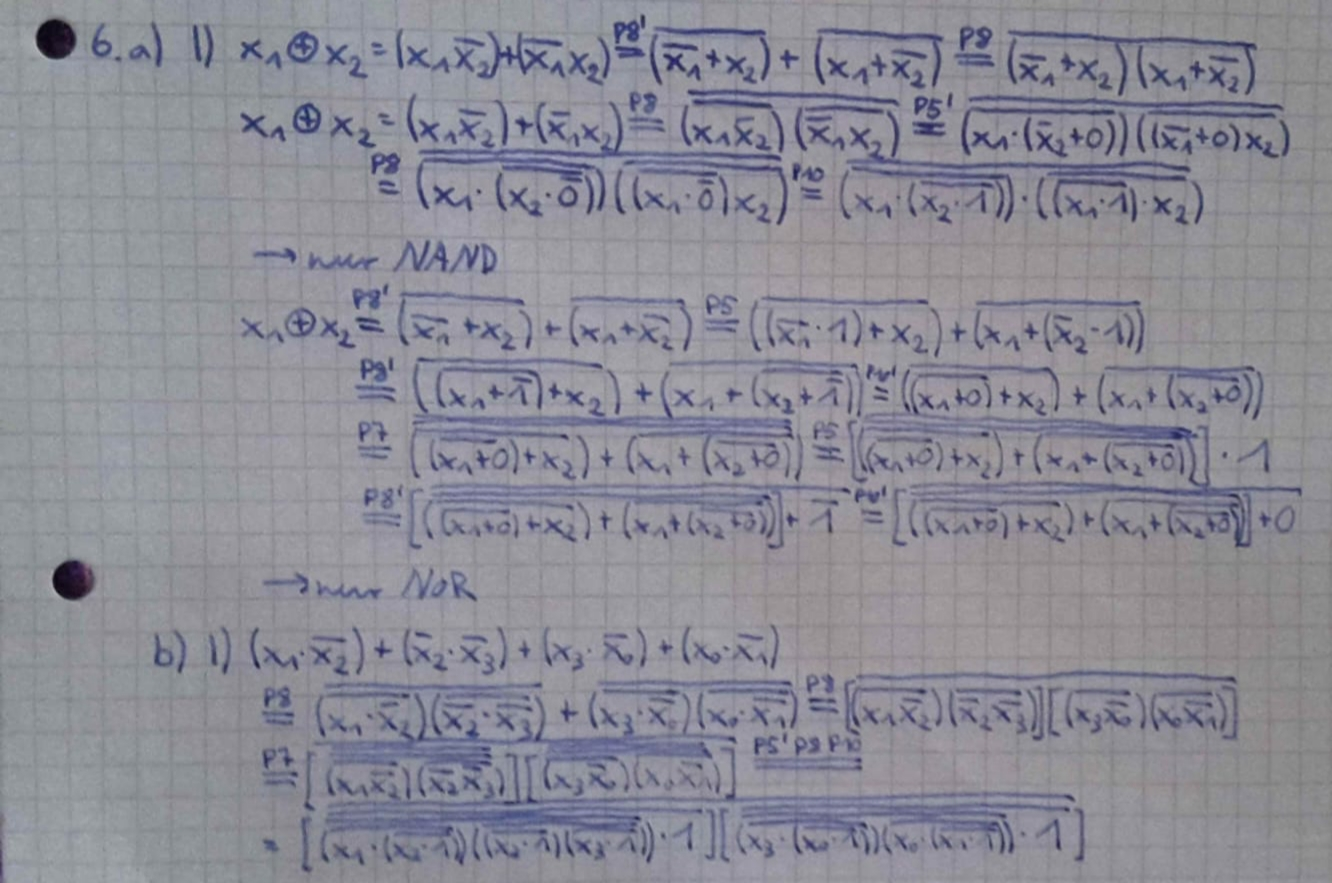
\includegraphics[width=\textwidth]{image.jpg}
    \caption{Aufabe 6}
\end{figure}
\end{document}
